\chapter{Implementation: Frontend}
\label{chapter:implementation-frontend}

To create an application that integrates into daily life, we will use the Flutter technology stack to develop software accessible across multiple platforms. For development, we have focused on optimizing the application for Android mobile phones. However, if we decide to expand the application to other platforms, it would require minimal additional work.

\begin{figure}[!ht]
	\centering
	\resizebox{0.5\textwidth}{!}{%
		\begin{circuitikz}
			\tikzstyle{every node}=[font=\Large]
			\draw [ rounded corners = 19.2] (3.25,5) rectangle (19.5,14.75);
			\draw  (3.75,5.5) -- (9.25,5.5) -- (9.75,8) -- (4.25,8) -- cycle;
			\node [font=\LARGE] at (6.75,6.75) {DetailsView};
			\draw  (12.75,5.5) -- (18.25,5.5) -- (18.75,8) -- (13.25,8) -- cycle;
			\node [font=\LARGE] at (15.75,6.75) {ResultsView};
			\draw [->, >=Stealth] (9.5,6.75) -- (13,6.75)node[pos=0.5, fill=white]{Gift Information};
			\draw  (13,14) rectangle  node {\Large OpenAI API Manager} (18.5,11.25);
			\draw [->, >=Stealth] (15,8) -- (15,11.25)node[pos=0.3, fill=white]{Gift Information};
			\draw [->, >=Stealth] (16.75,11.25) -- (16.75,8)node[pos=0.25, fill=white]{UI Gift Components};
			\node [font=\Large] at (6,14) {Flutter Android App};
			\draw  (15.75,19) ellipse (3.75cm and 1.25cm) node {\Large OpenAI API} ;
			\node [font=\Large] at (11.5,9.75) {};
			\draw [->, >=Stealth] (15,14) -- (15,17.75)node[pos=0.45, fill=white]{User Request};
			\draw [->, >=Stealth] (16.75,17.75) -- (16.75,14)node[pos=0.3, fill=white]{JSON Response};
		\end{circuitikz}
	}%

	\caption{Planned architecture of the App}
	\label{fig:architecture}
\end{figure}

Figure~\ref{fig:architecture} describes the planned architecture of the Flutter App. It has two main screens, which the User is guided through:
\begin{enumerate}
	\item In the \texttt{DetailsView}, the User can specify different attributes about the Person they would like to gift something to (furthermore called the Recipient)
	\item As soon as the User submits the Information, all Gift Information is Passed to the \texttt{ResultsView}.
	\item The \texttt{ResultsView} passes the received Information to the API Manager, which converts it into a prompt, which is then sent to the OpenAI API.
	\item The OpenAI Assistant processes the Request and returns a Response in Form of a JSON Object. (For more details see Section~\ref{sec:backend})
	\item The API Manager receives the JSON Object, extracts the relevant Information and sends it to the \texttt{ResultsView} in Form of prebuilt widgets, where they are displayed to the User.
\end{enumerate}

\section*{User Interface}

For the Design, we wanted a simple but clear User Interface. We used the \href{https://m3.material.io/}{Material Design Guidelines} to ensure a consistent Design. At first, we created a basic UI to test the app's core functionality. After developing the initial version of the app, we proceeded to validate the API Manager's ability to convert JSON responses into visually appealing Widgets.

Once the functionality had been confirmed, we focused on refining the User Interface. While not the primary objective of our project, we recognized that an improved UI can significantly enhance the overall user experience. We therefore implemented the following changes:

\begin{itemize}
\item A small infobox which instructs potential first-time users.
\item Improved display of input fields for age and hobbies.
\item The option to specify the Gender when selecting "Other".
\item Added titles for each Gift Idea to improve overview.
\item A button to instantly search for a gift on \url{galaxus.ch}
\end{itemize}

\begin{figure}[!h]

	\begin{subfigure}{0.5\textwidth}
		\begin{center}
			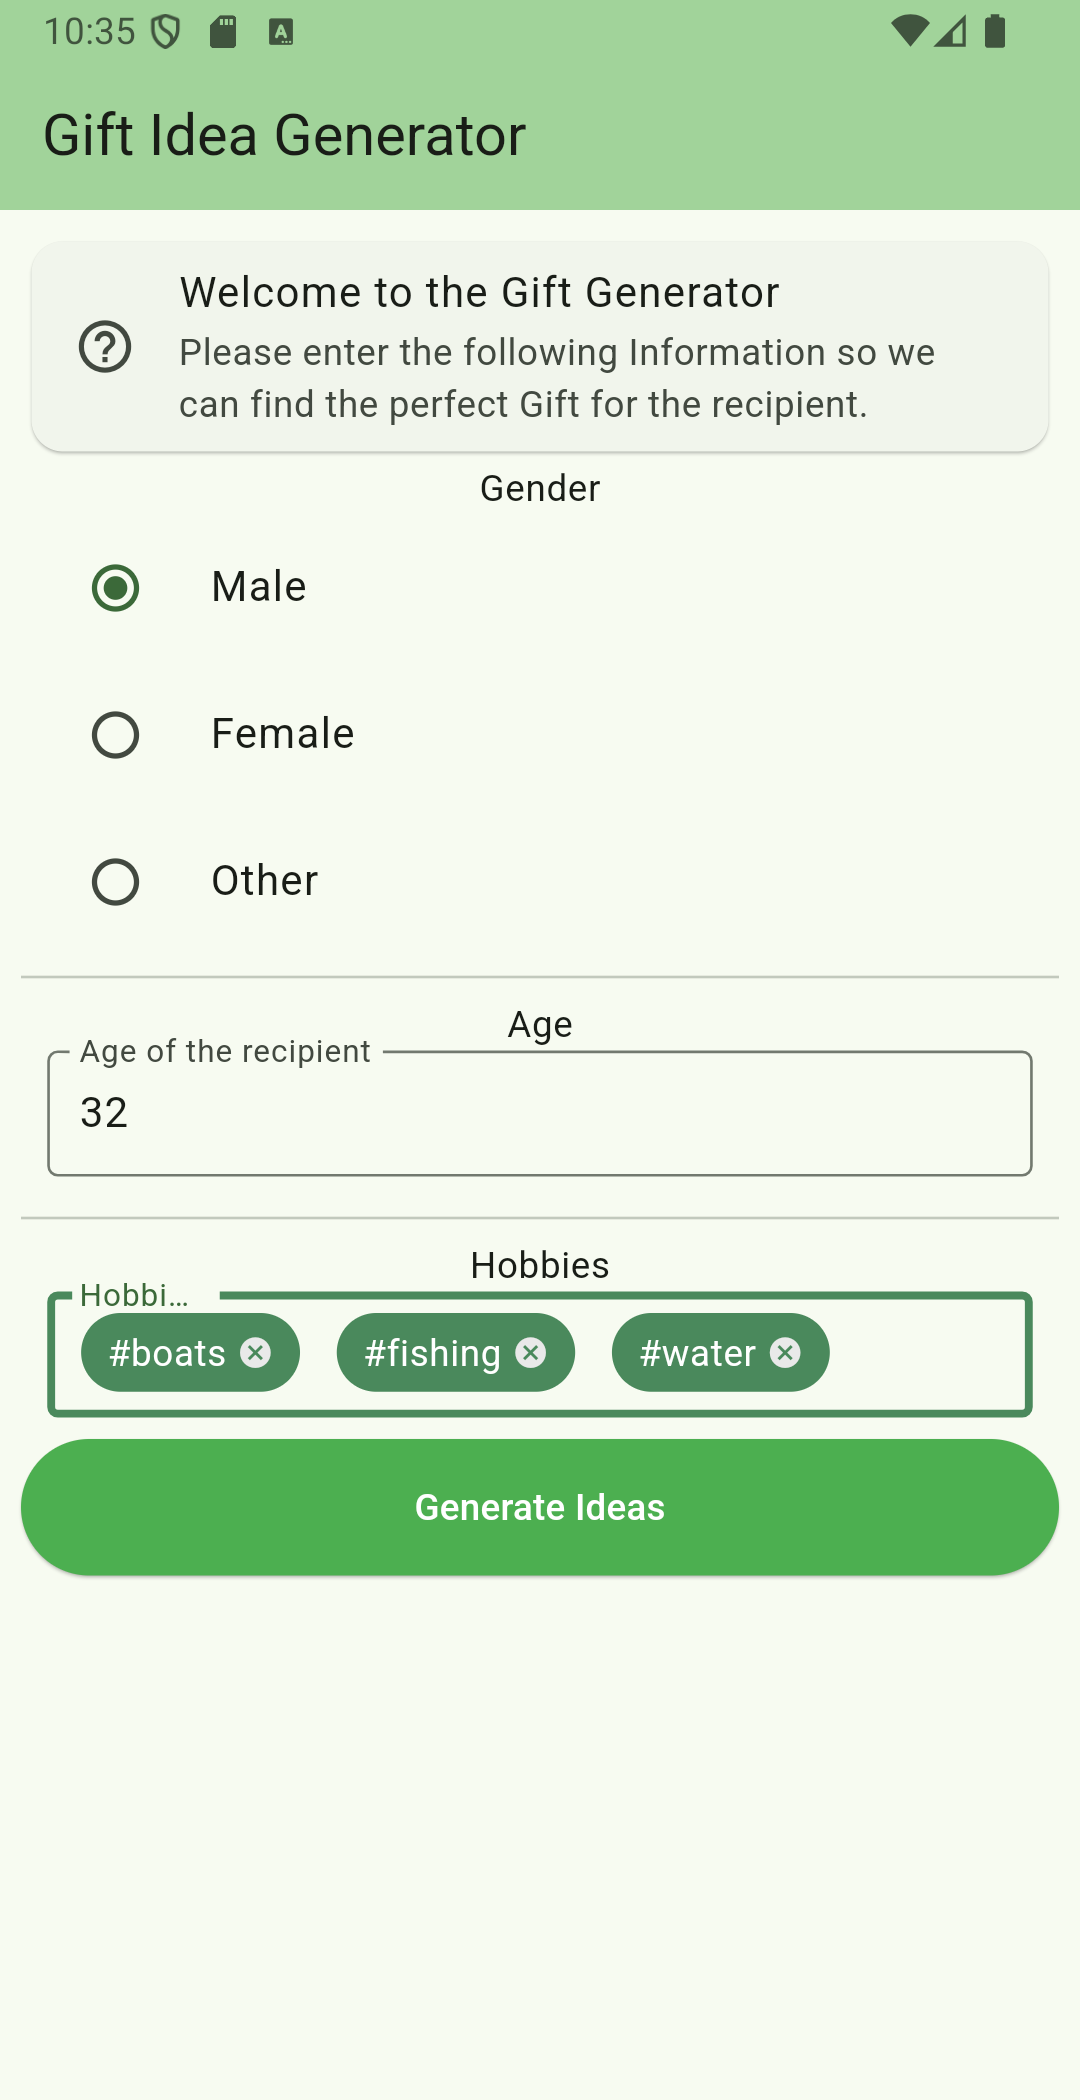
\includegraphics[height=7cm]{figures/screenshots/new_details_view_cropped.png}
		\end{center}
		\caption{\texttt{DetailsView}}
	\end{subfigure}
	\begin{subfigure}{0.5\textwidth}
		\begin{center}
			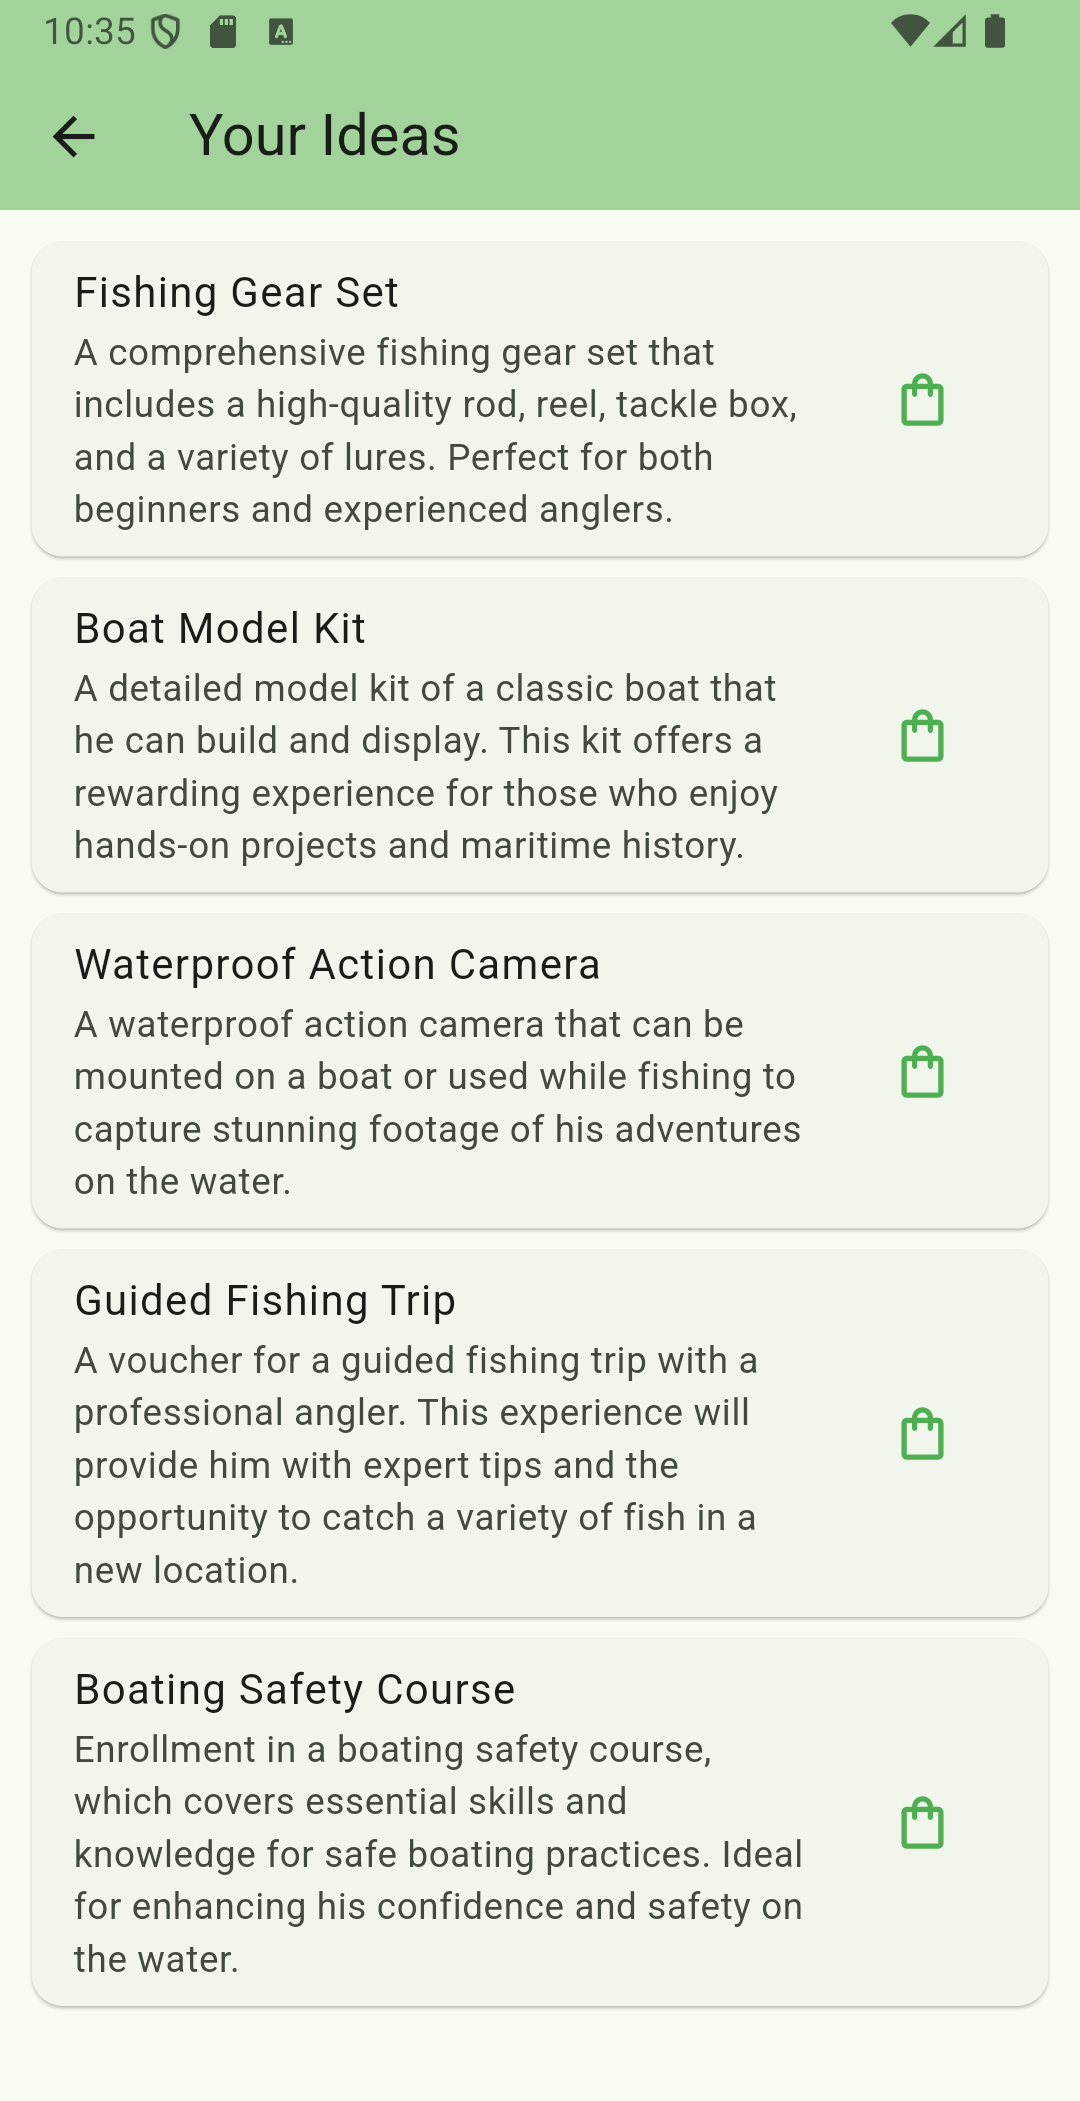
\includegraphics[height=7cm]{figures/screenshots/new_results_view_cropped.png}
		\end{center}
		\caption{\texttt{ResultsView}}
	\end{subfigure}
	\caption{Final Version of the Application}
	\label{fig:finalVersion}
\end{figure}

\section*{OpenAI API Manager}

The \texttt{OpenAI API Manager} is the backend logic which allows the Application to communicate with the OpenAI Assistant. It provides the functionality to convert User Input into a usable text prompt, as well as convert the received JSON into a user-friendly interface.

\begin{figure}[!h]
	\begin{lstlisting}[language=Java]
    factory GiftResponse.fromJson(Map<String, dynamic> data) {
        GiftResponse gr = GiftResponse();
        for (Map<String, dynamic> idea in data['presents']) { // Extract "present" objects
          gr.ideas.add(Idea(idea["title"], idea['description'])); // Fill information into new Idea() Object
        }
        return gr; // Return a GiftResponse() Object containing Ideas()
    }


    List<Widget> cards(Set<Idea> ideas) {
        List<Widget> cards = List.empty(growable: true);
        for (Idea idea in ideas) { // For all Ideas in the List
            cards.add(Card( // Add a new widget (Flutter Card Widget in this Case)
            child: ListTile(
                title: Text(idea.title), // Title
                subtitle: Text(idea.description), // Description
                trailing: IconButton( // Shopping Bag Button
                    onPressed: () {
                        _launchUrl(
                            "https://www.galaxus.ch/de/search?searchSectors=0&q=${idea.title}");
                    },
                    icon: Icon(Icons.shopping_bag_outlined, color: Colors.green,))),
            ));
        }
        return cards;
    }
\end{lstlisting}
	\caption{Code section responsible for converting JSON into Widgets}
\end{figure}
